% !TEX root = Master.tex

The same procedure as in Subsection \ref{sssec:margin_kcc_6} for key category cluster 2 will be applied here to analyze the marginal distribution of the log-sales in key category cluster 6.\\

Excluding all covariates, simple maximum likelihood estimation results can be summarized within \autoref{tab:estimated_parameters_kcc_6_no_covariates}, \autoref{fig:kcc_6_marginal} and \autoref{fig:res_kcc_6_no_covariates}. A Shapiro-Wilk test on the residuals returns a p-value of 0.87 and the fails to reject the null hypothesis of non-normality.
\\



\begin{table}[H]
\setlength\arrayrulewidth{1pt}  
\centering
\begin{adjustbox}{max width=\textwidth}\
\begin{tabular}{|c|c|c|}
\hline
\rowcolor{lightgray} 
$\hat{\mu}$ & $\hat{\sigma}$ & $\hat{\nu}$ \\ \hline
9.62        & 0.20           & 0.41        \\ \hline
\end{tabular}
\end{adjustbox}
\caption{Estimated parameters for log-sales of KCC 6 fitted to ex-Gaussian distribution with no covariate effects}
\label{tab:estimated_parameters_kcc_6_no_covariates}
\end{table}



 \begin{figure}[H]
\centering
\begin{subfigure}{.45\textwidth}
  \centering
  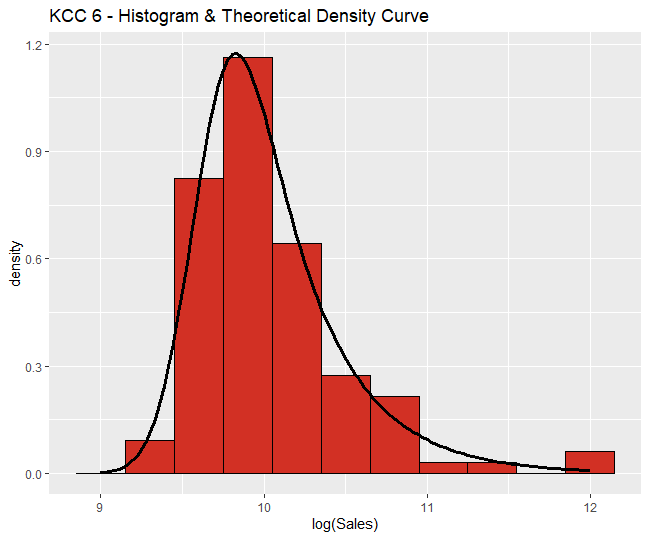
\includegraphics[width=\linewidth]{figures/kcc_6_density.png}
  \caption{Histogram \& theoretical density}
  \label{fig:kcc_6_density}
\end{subfigure}
\begin{subfigure}{.45\textwidth}
  \centering
  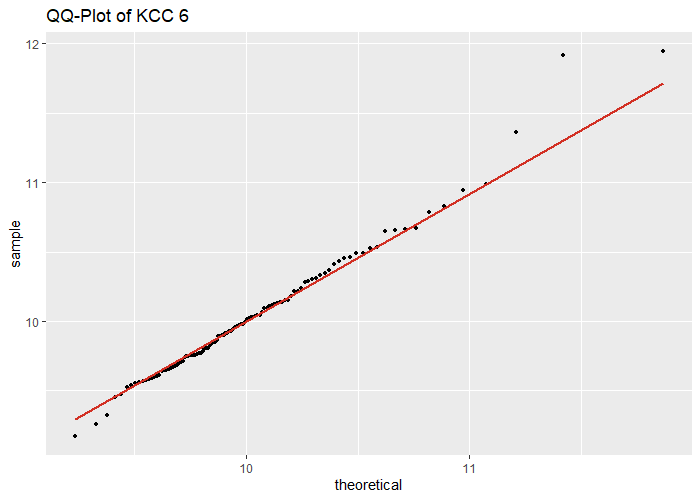
\includegraphics[width=\linewidth]{figures/kcc_6_qqplot.png}
  \caption{QQ-Plot}
  \label{fig:kcc_6_qqplot}
\end{subfigure}
\caption{ex-Gaussian distribution fitted to log-sales of \ac{KCC} 6}
\label{fig:kcc_6_marginal}
\end{figure} 


\begin{figure}[H]
\centering
  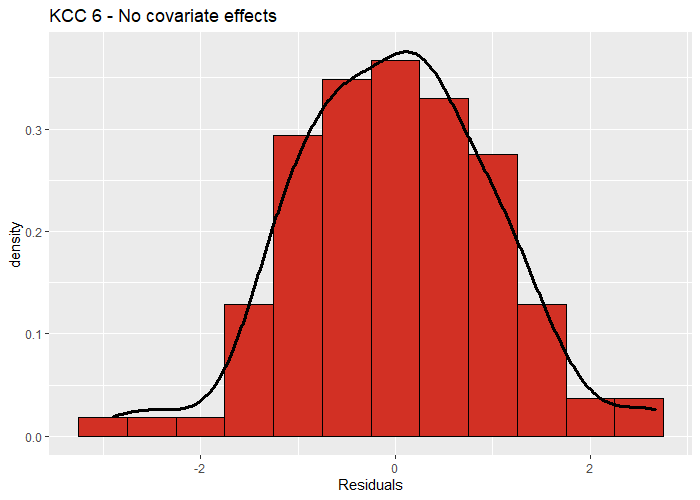
\includegraphics[width=0.45\linewidth]{figures/res_kcc_6_no_covariates.png}
  \caption{Residuals of KCC 6 log-sales fitted to an ex-Gaussian distribution with no covariate effects together with their density curve}
  \label{fig:res_kcc_6_no_covariates}
\end{figure}


Reviewing different model specifications, an equivalent model as in the previous Subsection is chosen (Model \ref{eq:gamlss_kcc_2}) with an ex-Gaussian distribution family for the response variable. A summary is printed below in R output \ref{output:gamlss_fit_kcc_6_try1}.
The estimated time-varying location and scale parameters can be seen in \autoref{fig:gamlss_kcc_6_estimated_parameters} and the skewness parameter $\hat{\nu}$ with 95\% CI in \autoref{tab:nu_ci_kcc_6}. Fitted values are close to real values, capturing the promotion peaks fairly well. The standard deviation fluctuates throughout time within a range between 0.1 and 0.3.
\\


%\VerbatimInput[frame = single, label = "GAMLSS Fit on KCC 6" ]{gamlss_fit_kcc_6_try1.txt}

\inputRoutput[caption={GAMLSS Fit on KCC 6}, numbers=left,numberstyle=\tiny, label=output:gamlss_fit_kcc_6_try1]{gamlss_fit_kcc_6_try1.txt}



\begin{figure}[H]
\centering
  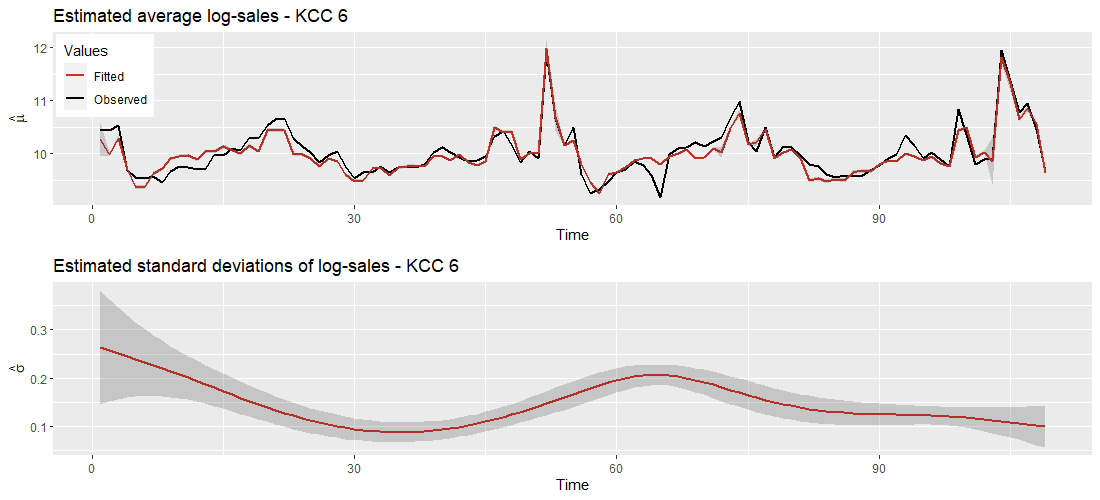
\includegraphics[width=0.95\linewidth]{figures/gamlss_kcc_6_estimated_parameters.png}
  \caption{Estimated location parameter $\hat{\mu}$ compared to the observed values and scale parameter $\hat{\sigma}$ with confidence bands of GAMLSS fit - KCC 6}
  \label{fig:gamlss_kcc_6_estimated_parameters}
\end{figure}



\begin{table}[H]
\setlength\arrayrulewidth{1pt}  
\centering
\begin{adjustbox}{max width=\textwidth}\
\begin{tabular}{|c|c|c|}
\hline
\rowcolor{lightgray} 
Lower & $\hat{\nu}$ & Upper \\ \hline
0.044        & 0.031           & 0.057        \\ \hline
\end{tabular}
\end{adjustbox}
\caption{Estimated skewness parameter $\hat{\nu}$ of GAMLSS fit with 95\% confidence interval bounds - KCC 6}
\label{tab:nu_ci_kcc_6}
\end{table}







\begin{figure}[H]
\centering
  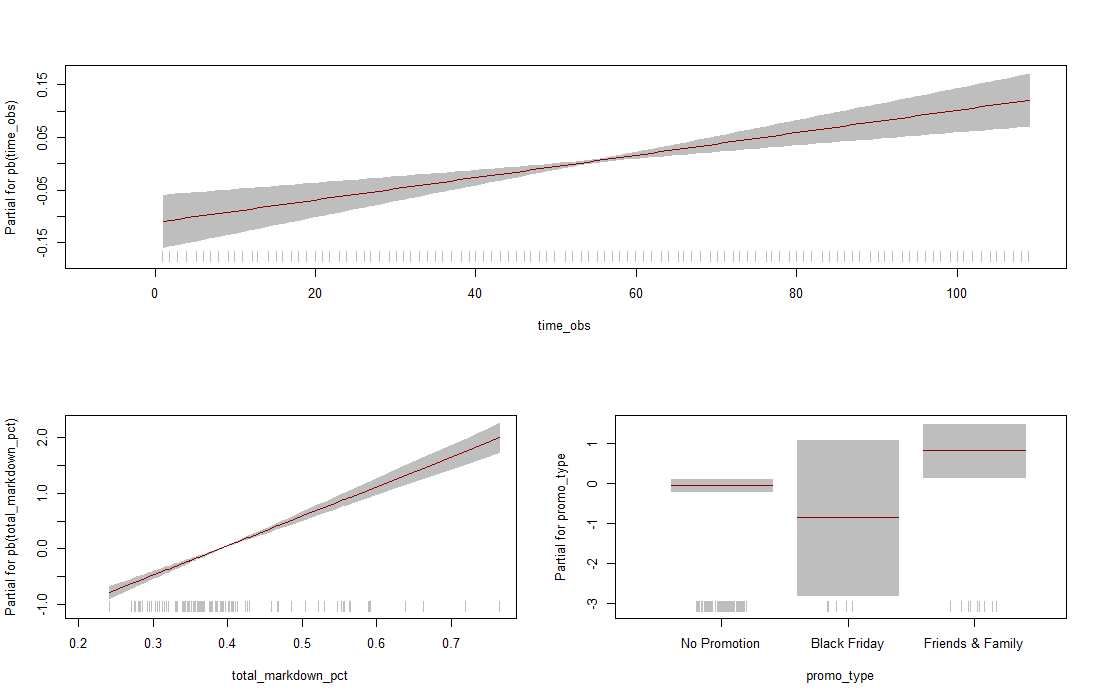
\includegraphics[width=0.95\linewidth]{figures/gamlss_effects_kcc_6.png}
  \caption{Covariate effects on the expected response variable (log-sales) of GAMLSS fit - KCC 6}
  \label{fig:gamlss_effects_kcc_6}
\end{figure}



\autoref{fig:gamlss_effects_kcc_6} reveals some interesting points regarding covariate effects. The temporal effect, just like the total markdown percentage, collapses to an increasing straight line. 
%The temporal effect also exhibits symmetrical behaviour around zero, including uncertainty. 
%Just like in \ac{KCC} 2, the effect of Spring-Summer is slightly smaller than that of Fall-Winter.
As opposed to the \ac{GAMLSS} fit for \ac{KCC} 2, Friends \& Family seems to have the highest effect of all promos for this \ac{KCC}. Controversial results are again the case here, as can be seen in R output \ref{output:gamlss_fit_kcc_6_try1}. The two promotions seem to negatively interact with the total markdown percentage. Those kinds of behaviour might need further investigation.
\\


Inspecting the diagnostic plots for the residuals in \autoref{fig:gamlss_residuals_kcc_6} along with the associated R output \ref{output:gamlss_residuals_kcc_6}, we can again confirm an appropriate fit. A Shapiro-Wilk test returns a p-value of 0.7, which is below the p-value of the fit without covariate effects. Nevertheless, normality is a steady assumption for the quantile residuals.
\\




\begin{figure}[H]
\centering
  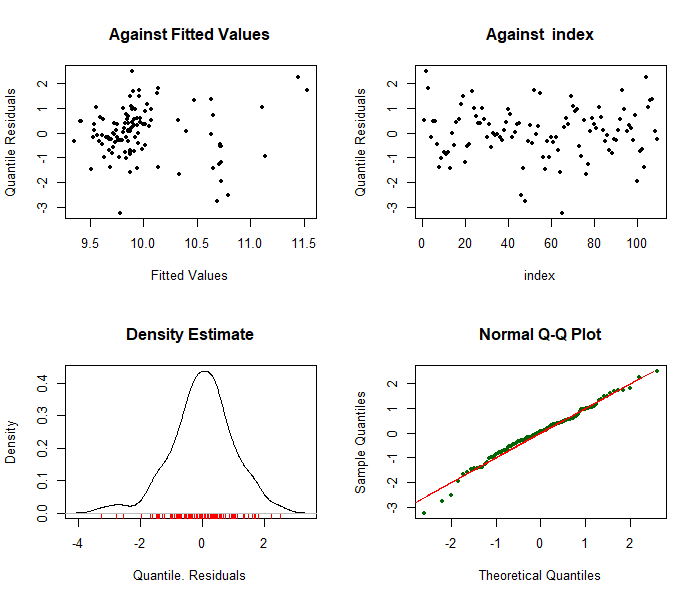
\includegraphics[width=0.95\linewidth]{figures/gamlss_residuals_kcc_6.png}
  \caption{Residuals of GAMLSS fit - KCC 6}
  \label{fig:gamlss_residuals_kcc_6}
\end{figure}


%\VerbatimInput[frame = single, label = "Residuals of GAMLSS Fit on KCC 6" ]{gamlss_residuals_kcc_6.txt}

\inputRoutput[caption={Residuals of GAMLSS Fit on KCC 6},numbers=left,numberstyle=\tiny, label=output:gamlss_residuals_kcc_6]{gamlss_residuals_kcc_6.txt}
















